\documentclass{article}

\usepackage[a4paper]{geometry}

%pseudocode:
\usepackage{algorithm}
\usepackage{algpseudocode} 

%figures:
\usepackage{tikz}
\usetikzlibrary{trees,positioning,backgrounds}
\usepackage{tikz-qtree}

%references and keeping floats in place
\usepackage{hyperref}
\usepackage[section]{placeins}

\title{Doubling \dops \\ 
{\normalsize Data Oriented Parsing based on \ddop~and \dops}}
\author{Benno Kruit (10576223)\\
Sara Veldhoen (10545298)}



\begin{document}
%NB: gebruik \dops{} of \dops~ om netjes een whitespace erachter te krijgen in lopende tekst
\newcommand{\dops}[0]{DOP$ ^*$}
\newcommand{\ddop}[0]{Double-DOP}


\maketitle

\section{Introduction}
%Introduction to the paper
%General introduction to the DOP framework, terminology 
%NB: introduce term 'fragment' for usage throughout this document



%Je hebt de introductie en terminologie helemaal uit elkaar getrokken. Wat op zich wel helder is, maar niet zo compact.. Aangezien we maar 9 pagina's mogen schrijven kunnen we dat denk ik beter samenvoegen.

\begin{figure}[h!]
\center \input{figureTreebank}
\caption{A toy treebank} \label{f:treebank}
\end{figure}

A common approach to natural language syntax, is to view the structure of sentences as constituent trees. An artificial example of a treebank is given in figure \ref{f:treebank}. Constituent trees can be described by a \emph{Context Free Grammars} (CFGs),  such that all trees are built up from  rules that each describe the production (children nodes) of a single node (parent) in the tree. When building an empirical model of observed parse trees, these rules are extended with probabilities to form a \emph{probabilistic CFG} (PCFG). This gives the trees that are `generated' by these rules their own probability, which makes it a statistical model of a distribution over natural language syntax.

The simple rules of a CFG cannot describe all linguistic phenomena, such as long distance dependencies. Grammars can be enriched by Markovisation, to include deeper levels in the tree. 


\subsection{DOP}
\emph{Data-Oriented Parsing} (DOP), as first introduced in \cite{scha1990}, takes a different approach. It models the language with a Probabilistic Tree Substitution Grammar (PTSG). 
The trees in the treebank are taken apart, which results in \emph{fragments} of arbitrary depth. 
A fragment is a connected subgraph of a tree such that it corresponds to context-free productions in that tree, i.e. each node must have either have children with the same labels as in the original tree, or no children at all. This is illustrated in figure \ref{f:fragments}. Note that a level-one fragment corresponds to a CFG rule. Its \emph{symbolic grammar} refers to the set of fragments (that receive a non-zero weight) in a grammar. 



\begin{figure}[h!]
\center 
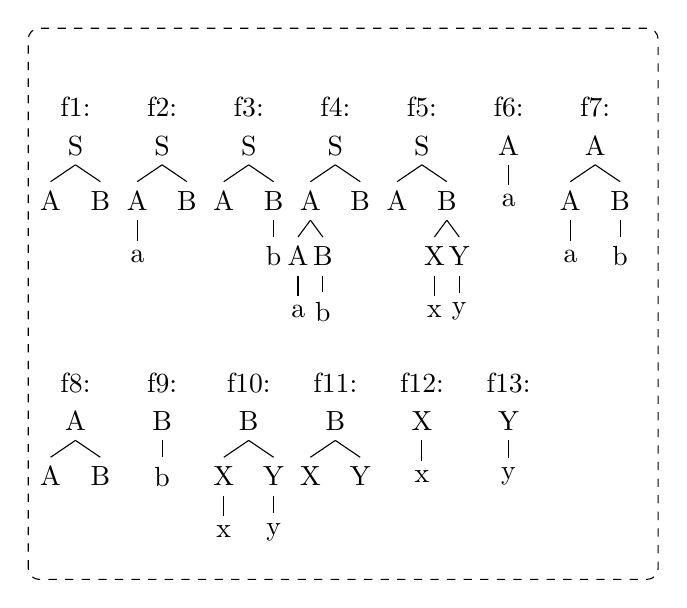
\begin{tikzpicture}
[node distance = 0 pt, sibling distance=18pt, level distance=20pt,level 2/.style={sibling distance=9pt},level 3/.style={sibling distance=9pt}]

\draw[black,dashed,join=round, inner frame sep=2cm and 2cm, rounded corners ] (0,3) rectangle (8,10);
%\node[fill = white, rectangle, draw] (treebank) at(3.5,10) {Fragments with non-zero weights};


\node (f1) at(0.6,9){f1:}
node [ below =of f1] {S}
child {node {A} 		}
child {node {B}		}
;


\node (f2) at(1.7,9){f2:}
node [ below =of f2] {S}
child {node {A} 	child {node {a}}
	}
child {node {B}	}
;

\node (f3)  at(2.8,9){f3:}
node [ below =of f3] {S}
child {node {A} 	}
child {node {B}	child{node {b}}
	}
;

\node (f4) at(3.9,9) {f4:}
node [ below =of f4] {S}
child {node {A} 	child{node {A}	child{node {a}}}
			child{node {B}	child{node {b}}}
	}
child {node {B}		}
;

\node (f5) at(5.0,9) {f5:}
node [ below =of f5] {S}
child {node {A} 		}
child {node {B}	child{node {X}	child{node {x}}}
			child{node {Y}	child{node {y}}}
	}
;

\node(f6) at(6.1,9) {f6:}
node [ below =of f6] {A}	
	child {node {a}}
;

\node(f7) at(7.2,9) {f7:}
node [ below =of f7]  {A} 	
	child{node {A}	child{node {a}}}
	child{node {B}	child{node {b}}}
;




\node(f8) at(0.6,5.5){f8:}
node [ below =of f8]  {A} 	
	child{node {A}	}
	child{node {B}	}
;

\node(f9) at(1.7,5.5) {f9:}
node [ below =of f9] {B}	
	child {node {b}}
;

\node(f10) at(2.8,5.5) {f10:}
node [ below =of f10]  {B} 	
	child{node {X}	child{node {x}}}
	child{node {Y}	child{node {y}}}
;

\node(f11) at(3.9,5.5) {f11:}
node [ below =of f11]  {B} 	
	child{node {X}	}
	child{node {Y}	}
;

\node(f12) at(5.0,5.5) {f12:}
node [ below =of f12] {X}	
	child {node {x}}
;

\node(f13) at(6.1,5.5) {f13:}
node [ below =of f13] {Y}	
	child {node {y}}
;
\end{tikzpicture}

\caption{All extracted fragments}
\label{f:fragments}
\end{figure}


Fragments can be combined in a \emph{derivation} to build syntactic structures. A step in a derivation is a composition, denoted by the symbol $\circ$. We follow the convention to only allow left-most derivations. This means that the left-most non-terminal node in a fragment $f_1$ must correspond to the root node of $f_2$ in order to derive $f_3=f_1\circ f_2$

For each fragment, the probability is estimated by counting how often it occurs in the treebank, compared to others with the same root. The probability of a derivation is the product of the probability of the fragments. Note that a single tree can be the result of different derivations. Therefore probability of a tree is the sum of the probabilities of all its derivations.

\subsection{Theoretical issues}
It has been argued that DOP (in its original formulation) is biased and inconsistent \cite{johnson2002}, both assumed to be bad properties of an estimator in general. As we will see, bias is not necessarily a bad thing. In fact, Zollman proves in  \cite{zollmann2005} that any non-overfitting estimator is biased. Furthermore, he shows that it is possible to define a DOP-estimator that is consistent.


\subsection{Practical issues}
In its original formulation, DOP takes the trees apart in all possible ways. The number of fragments is exponential in the length of the sentences, thus the size of the symbolic grammar would be far too huge to be computationally feasible. 
Different approaches have been taken to reduce the symbolic grammar, e.g. by sampling or by applying a smart algorithm. This appears to be far from trivial.


\subsection{Outlook}
Section~\ref{sec:Statistics} elaborates the notions of consistency and bias and their relation to overfitting.
In section~\ref{sec:Existing}, we outline two approaches that tackle the reduction of the symbolic grammars: \ddop{} and \dops{}. This report focuses on a comparison of these approaches. Theoretically, they differ in that \dops{}, unlike \ddop{}, has been proven to be consistent \cite{zollmann2005}. We investigate the differences between the grammars produced by \ddop{} \dops{}. The algorithms can be decomposed into two parts. We also analyze the impact of the partial choices by mutually using these parts.

Section~\ref{sec:Comparison} offers a detailed comparison of the two methods as well as a description of the experiments we conduct. In section~\ref{sec:Results}, we present our findings and provide an analysis. 




\section{Existing Frameworks: Double-DOP and DOP$^*$}
%A description and comparison of Double-DOP and DOP*

A PTSG consists of the symbolic grammmar, i.e. a set of fragments, and the corresponding weights. In the general case of DOP, all fragments are extracted from all the trees in the treebank. The number of fragments is exponential in the length of the sentences, thus the total number of fragments extracted would be far too large for efficient computation. 
%DOP1: sample
Later models have therefore restricted the set of fragments in the grammar, thus improving computational efficiency. However, determining a proper subset of fragments to use is not trivial and this choice may negatively influence the performance of the grammar.

%Iets met Goodman? Die behoudt alleen kleine stukjes en speciale regels, maar daardoor geen expliciete representatie van 'productive units' (Sangati, einde van sectie 2)

In this section, we outline two approaches to constrain the extraction of fragments: \ddop and \dops. Furthermore, we discuss the similarities and dissimilarities for these two approaches. 

\subsection{\ddop}
In the following, we discuss \ddop{} as it was presented in \cite{sangati2011}. In this model, no unique fragments are extracted from the dataset: if a construction occurs in one tree only, it is probably not representative for the language. This is carried out by a dynamic algorithm using tree-kernels. It iterates over pairs of trees in the treebank, looking for fragments they have in common. In addition, only the largest shared fragment is stored. 

The symbolic grammar that is the output of this algorithmis not guaranteed to derive each tree in the training corpus. Therefore all one-level fragments, consitutuing the set of PCFG-productions, are also added.

After the extraction of the symbolic grammar, the weights are obtained. This is done in a second pass over the treebank, assessing the relative frequencies. 

The \ddop{} model has its main focus on determining the symbolic grammar. However, it was implemented with different estimators and maximizing objectives. Empirical results show that %

\paragraph{Consistency and bias}

\subsection{\dops}
In \dops{} \cite{zollmann2005}, a rather different approach is taken called held-out estimation. The treebank is split in two parts, the extraction corpus ($EC$) and a held-out corpus ($HC$). An initial set of fragments is extracted from the $EC$, containing all the fragments from its trees. The weights are then determined so as to to maximize the likelihood of $HC$, under the assumption that this is equivalent to maximizing the joint probability of the \emph{shortest derivations} of the trees in $HC$. All fragments that do not occur in such a derivation are removed from the symbolic grammar. Note that some trees in $HC$ may not be derivable at all. 

\paragraph{Consistency and bias}
\dops{} was claimed to be the first consistent (non-trivial) DOP-estimator, \cite{zollmann2005} provides a consistency proof. On the other hand \dops{} is  biased, but Zollmann shows how bias actually arises from generalization: no non-overfitting DOP estimator could be unbiased. Bias is therefore not prohibited but on the contrary a desirable property of an estimator.

In \cite{zuidema2006} it is argued that there is a problem with the consistency proof given for \dops{}, as well as the non-consistency proof for other DOP-estimators by \cite{johnson2002}. Zuidema points out that these proofs use a frequency-distribution test, whereas for DOP a weight-distribution test would be more appropriate. 
%Wat hiermee?

%
%\subsection{Comparison}
%Both \dops{} and \ddop{} restrict the symbolic grammar based on some notion of reoccurence of fragments. 
%
%In \ddop{} this is evident, it is explicit in the algorithm how (largest) reoccuring fragments are added to the grammar. From a computational point of view, this approach is very intuitive and can be implemented rather efficiently. However, the threshold (two) on the number of reoccurences might seem rather trivial. Indeed, \cite{sangati2011} reports experiments varying this threshold that show how performance drops for higher thresholds, with on the other hand a great reduction of the size of the grammar. A proper setting might well depend on the size and nature of the treebank used, and the computational costs one is willing to pay. In short, \ddop{} is computationally attractive but its theoretical foundation is not convincing us.
%%wel performance maar competence raadsel
%
%Theoretically,\dops{} is more appealing: we decide on the symbolic grammar by assessing which fragments are actually used in derivations. The main assumption is that shortest derivations are preferred. The splitting of the treebank makes this possible (otherwise the grammar would be terribly overfitted).
%
%
%
%\subsection{Preview}
%\dops{} is proven to be consistent and theoretically appealing. The computational problem of \dops{} is that, at first, the entire set of possible fragments is extracted from $EC$ and this set is reduced in a later phase. This comes with the need for huge storage and computation. In the next section, we investigate the possibility of reformulating the \dops{} approach with insights from the \ddop{} model to maintain the best of both worlds. 
%
%%\dops{} theoretically more appealing, \ddop{} computationally: lend properties of \ddop{} to implement \dops{}






\subsection{Comparison}
%The theoretical properties of \dops{} and \ddop{} differ:  
\dops{} and \ddop{} differ both in the set of fragments they extract and their estimation of the weights. To investigate the exact differences, we will view both steps separately.

Note that the \dops{} extraction needs another decision: in many cases, there are several shortest derivations possible. From now on, we add all fragments that occur in one of these shortest derivations to the symbolic grammar. Of course we need to adjust the weights (e.g. divide the frequency counts by the number of shortest derivations) so that no full tree gets a higher impact on the PTSG. We will keep to the original formulation of \dops{} in case no derivation is possible, i.e. not including any fragments for this tree.

\paragraph{Extraction}
\ddop{} uses tree kernels to find the maximal overlapping fragments of pairs of trees, which are added to the symbolic grammar. We will call this the \emph{maximal-overlap} method. \dops{} iteratively finds the shortest derivation of one tree given all the fragments of a set of trees, herafter the \emph{shortest-derivation} method. The example in figure \ref{f:differentSets} shows that the sets of extracted fragments from these methods does indeed differ.

\begin{figure}
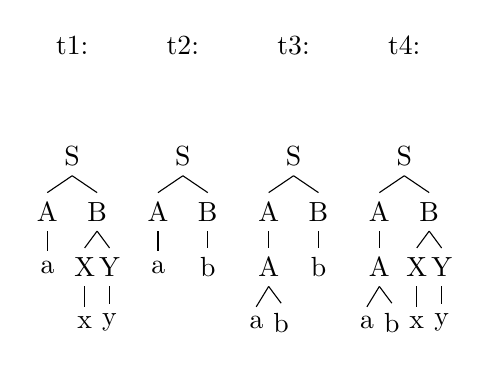
\begin{tikzpicture}
[node distance = 40 pt, sibling distance=18pt, level distance=20pt,level 2/.style={sibling distance=9pt},level 3/.style={sibling distance=9pt}]

\node (t1) {t1:}
node [ below of= t1] {S}
child {node {A} 	child {node {a}}
	}
child {node {B}	child{node {X}	child{node {x}}}
			child{node {Y}	child{node {y}}}
	}
;

\node [right of = t1] (t2) {t2:}
node [ below of= t2] {S}
child {node {A} 	child {node {a}}
	}
child {node {B}	child{node {b}}
	}
;

\node [right of = t2] (t3) {t3:}
node [ below of= t3] {S}
child {node {A} 	child {node {A}	child{node {a}}
						child{node {b}}
				}
	}
child {node {B}	child{node {b}}
	}
; 

\node [right of = t3] (t4) {t4:}
node [ below of= t4] {S}
child {node {A} 	child {node {A}	child{node {a}}
						child{node {b}}
				}
	}
child {node {B}	child{node {X}	child{node {x}}}
			child{node {Y}	child{node {y}}}
	}
;
\end{tikzpicture}
\caption{The fragment sets resulting from \emph{maximal-overlap} and \emph{shortest-derivation} extraction}
\label{f:differentSets}
\end{figure}

It is easy to see that the \dops{} extraction method does not depend on the corpus split: we can also try to find the shortest possble derivation using fragments from all the other trees. Likewise \ddop{} could be implemented using a split, comparing pairs that consist of a tree from each part of the corpus. Whether the corpus is split in two does only influence the size of the symbolic grammar and not its constitution.

Therefore, we will implement both extraction methods in a 1 vs the rest manner. In this way, we can analyse how the resulting symbolic grammars differ. The analysis will comprise the size of the resulting symbolic grammar and the relative number of fragments of certain depth. Furthermore, we might be able to find interesting patterns by manually looking at the fragments that were extracted by one of the systems only.s

\paragraph{Estimation}
The next step would be to compare the estimation methods: use either a split or the whole set of trees for both estimators. \ddop{} counts the occurences of fragments in the symbolic grammar, whereas \dops{} counts the occurrences in shortest derivations. Therefore, the extraction and estimation are best done simultaneously in the latter case. This comparison would involve a performance measure, such as the F1-score for correctly predicted parses.





























\section{Implementation}
%Description of our implementation, how does it resemble Double-DOP and DOP*? What are the differences? What are the theoretical capabilities? 

\subsection{Extraction}
Algorithm \ref{a:dops2} performs shortest-derivation extraction (as in \dops{}) in an efficient way, resembling the tree kernel approach in the iterative comparison of one tree with others. Namely, we iterate over the trees in $HC$ (lines 2-8): create a list $F$ of all of its fragments that occur in the rest of the treebank (line 3) and increment the count of the fragments in $F$ that occur in the shortest derivation(s). In this way, we do not need to store all fragments in $EC$ as in the initial step of the original \dops{} algorithm. 

Algorithm \ref{a:ddop1} performs the maximal-overlap extraction (as in \ddop{}). For the comparison of trees to find the maximal overlap (line 4), the tree kernel approach from \cite{sangati2011} is used. 

\begin{algorithm}
{\bf Data}: a treebank $TB$\\
{\bf Result}: a map of tree fragments and corresponding counts in shortest derivations\\
\begin{algorithmic}[1]
\State{Initialize $M$, a map from fragments to counts, empty}
\For {$t\in TB$}
	\State $F \gets Frag(t)\cap \bigcup\limits_{t'\in TB/\{t\}} frag(t')$
	\State{$D\gets$ the shortest derivation(s) of $t$ using fragments in $F$}		
	\For{$f\in D$}
		\State add $f$ to $M$ {\bf if} $f\not\in M$
		\State $M[f]\gets M[f]+1$ \Comment{Anticipating the estimation step}
	\EndFor
\EndFor
%\For{$n \in V_N$}
%	\State{Add the counts of all fragments rooted at $n$}
%	\State{Normalize the weights of these fragments}
%\EndFor	
\end{algorithmic}
\caption{Shortest derivation extraction in a one vs the rest manner}
\label{a:dops2}
\end{algorithm}


\begin{algorithm}
{\bf Data}: a treebank $TB$\\
{\bf Result}: a set of tree fragments\\
\begin{algorithmic}[1]
\State{Initialize $M$, a map from fragments to weights, empty}
\For{$t\in TB$}
	\For{$t'\in TB/\{t\}$}
		\State $f\gets$ maximal overlapping fragment(s) of $t$ and $t'$
		\State add $f$ to $M$ {\bf if} $f\not\in M$
	\EndFor
\EndFor
\end{algorithmic}



\caption{Maximal overlap extraction in a one vs the rest manner}
\label{a:ddop1}
\end{algorithm}

\subsection{Estimation}
Now for estimation, we use the output of the extraction algorithm. In the case of shortest-derivation extraction (algorithm \ref{a:dops2}), we only need to normalize the counts in $M$ to their relative frequency as compared to fragments that have the same root. In the case of maximal-overlap extraction (algorithm \ref{a:ddop1}), we need to iterate over the dataset once more to count the occurences of the fragments in the output and then compute their relative frequencies.

%In \ddop, we would iterate over pairs of trees. With treebank size $n$, that would require $n!$ comparisons. In our proposed algorithm, we need to iterate over each combination of a tree in $HC$ with (worst case\footnote{The condition in line $5$ avoids unnecessary search for fragments. We might be able to pose a smarter constraint here, such that we only continue if we can possibly find fragments that lead to a shorter derivation}) all trees in $EC$. This requires $n/2 \times n/2$ comparisons. Furthermore, we immediately store the counts, so we don't need to iterate over the data again to assess the weights. We do however need to normalize the weights, such that the sum of weights of all fragment sharing the same root equals 1.




%In words: Iterate over the trees in $HC$ (lines 2-17): create a list $F$ of all of its fragments that occur in $EC$ (lines 3-12). This procedure resembles the treekernels from \ddop. Create the shortest derivation $D$ from fragments in $F$ (NB: this is not always possible, in which case $D=\emptyset$). Increment the counts of these fragments in the map $M$

%\begin{algorithm}[H]
%{\bf Data}: non-overlapping treebanks $EC$ and $HC$\\
%{\bf Result}: a PTSG, i.e. a map of tree fragments and corresponding weights\\
%\begin{algorithmic}[1]
%\State{Initialize $M$, a map from fragments to weights, empty}
%\For {$t_H\in HC$}
%%	\State $Q\gets frag(t_H)$
%%	\State $F \gets \emptyset$
%%	\While{$Q$ not empty}% or a smarter constraint
%%		\For{$t_E \in EC$}
%%			\For{$f \in Q\cap frag(t_E)$}
%%				\State $Q\gets Q/\{f\}$	
%%				\State $F\gets F\cup\{f\}$	
%%			\EndFor
%%		\EndFor
%%	\EndWhile
%	\State $F \gets Frag(t_H)\cap \bigcup\limits_{t_E\in EC} frag(t_E)$
%	\State{$D\gets$ the shortest derivation of $t_H$ using fragments in $F$}		
%	\For{$f\in D$}
%		\State add $f$ to $M$ {\bf if} $f\not\in M$
%		\State $M[f]\gets M[f]+1$
%	\EndFor
%\EndFor
%\For{$n \in V_N$}
%	\State{Add the counts of all fragments rooted at $n$}
%	\State{Normalize the weights of these fragments}
%\EndFor	
%\end{algorithmic}
%\caption{\dops{} extraction and estimation}
%\label{a:dops1}
%\end{algorithm}
\section{Results}\label{sec:Results}
%Empirical results of our implementation (on the WSJ corpus?)

\begin{figure}
\center
\includegraphics[width=\linewidth]{../data/plots/plot0.png}
\end{figure}


\begin{figure}
\center
\includegraphics[width=\linewidth]{../data/plots/plot1.png}
\end{figure}


\begin{figure}
\center
\includegraphics[width=\linewidth]{../data/plots/plot2.png}
\end{figure}


\begin{figure}
\center
\includegraphics[width=\linewidth]{../data/plots/plot3.png}
\end{figure}
\section{Conclusion}
%Discussion, future work

%Split (held-out est) reduces bias towards large fragments


%Double-DOP: best performance

%Performance not correlated with consistency of the method

%Shortest derivation, very short grammar. But not as useful as it would seem: bad performance

\paragraph{Future work}
% analysis of other DOP grammars, 
%more elaborate analysis: possibly clustering on features such as depth, number of substitution sites and terminals

% is consistency indeed a valuable property at all?



\bibliographystyle{ieeetr}
\bibliography{bibliography}

\end{document}
